\chapter{Results and Discussions}

This chapter presents the outcomes of implementing and testing Project Koschei --- a 3D first-person multiplayer social deduction game set in a fictionalised Chernobyl Exclusion Zone, powered by a memory-augmented Large Language Model (LLM) acting as an alien impostor. The results are evaluated across four primary dimensions: user interface and session flow, in-game systems and world design, LLM-driven deception behaviour, and combat encounters. Observations are discussed in the context of the design goals outlined in earlier chapters.

% -------------------------------------------------------
\section{User Interface and Session Flow}

\subsection{Login Screen}

The game launches into an atmospheric login screen rendered with dark, fog-drenched environmental art consistent with the Chernobyl setting. Players are presented with a single \textit{Username} input field and a \textit{Play Game} button styled in deep red, immediately establishing the game's tone. An \textit{Exit Game} button is available in the lower-right corner. The minimalist interface ensures fast entry into the game session without unnecessary friction.

\begin{figure}[h]
    \centering
    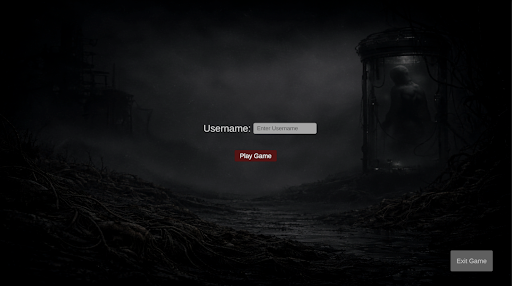
\includegraphics[width=0.85\textwidth]{Images/login.png}
    \caption{Login screen of Project Koschei featuring a username entry field and \textit{Play Game} button, set against a dark, atmospheric background with a looming hourglass figure.}
    \label{fig:login}
\end{figure}

\subsection{Multiplayer Lobby}

Upon login, players are placed in a lobby screen showing a countdown timer (\textit{Time Left}) and the lobby name. Connected players are listed by username --- as seen with players \textit{noobmaster99} and \textit{goober} --- in a clean dark-themed list. A \textit{Leave Lobby} button and a \textit{Start Game} button are positioned at the lower-left and lower-right respectively, giving the host control over round initiation.

\begin{figure}[h]
    \centering
    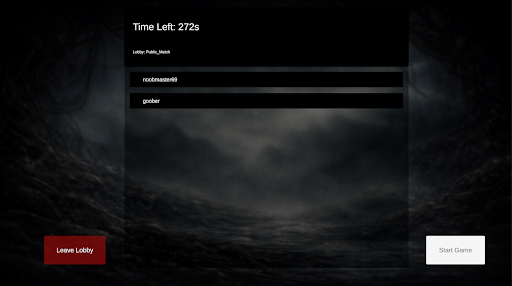
\includegraphics[width=0.85\textwidth]{Images/lobby.png}
    \caption{Multiplayer lobby interface displaying connected players (\textit{noobmaster99}, \textit{goober}), a countdown timer, and round start controls.}
    \label{fig:lobby}
\end{figure}

% -------------------------------------------------------
\section{In-Game Systems}

\subsection{HUD and World Environment}

The in-game HUD displays essential player information at the screen edges: ammo count (30/30) in the top-right, player health (100/100) as a red bar at the bottom-centre, and an equipment slot labelled \textit{Empty} with an \textit{[E] Pick Up} prompt. The game world features an open outdoor environment with dense vegetation, a distant watchtower, wooden structures, and a misty skyline, faithfully evoking the abandoned Soviet exclusion zone aesthetic.

\begin{figure}[h]
    \centering
    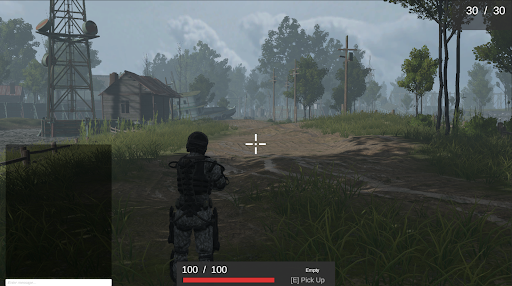
\includegraphics[width=0.85\textwidth]{Images/hud.png}
    \caption{In-game HUD showing ammo (30/30), health bar (100/100), and item pick-up prompt, with the exclusion zone environment visible in the background.}
    \label{fig:hud}
\end{figure}

\subsection{NPC Researcher Interaction}

Players can approach NPC researchers stationed throughout the map to receive contextual information. As shown in Figure~\ref{fig:npc_interaction}, three characters --- two armed soldiers and one NPC in a blue hazmat suit --- are gathered near a wooden structure. The NPC delivers narrative dialogue displayed in a subtitle bar at the bottom of the screen: \textit{``I am what remains of the advance team. We entered three days ago. There were four of us. Now there is me.''} This interaction system grounds the lore and provides players with investigative leads.

\begin{figure}[h]
    \centering
    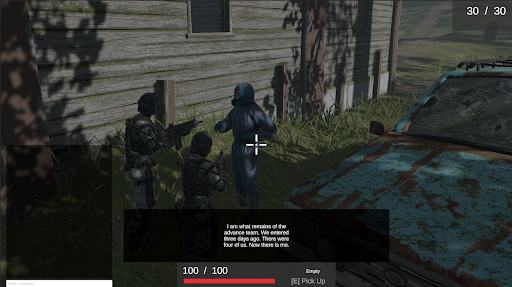
\includegraphics[width=0.85\textwidth]{Images/npc_interaction.png}
    \caption{Player interacting with an NPC researcher in a blue hazmat suit. The NPC delivers survival lore via the in-game subtitle system, revealing that the advance team has been largely eliminated.}
    \label{fig:npc_interaction}
\end{figure}

% -------------------------------------------------------
\section{LLM-Driven Deception and Proximity Chat}

\subsection{Impostor Chat in Gameplay}

The proximity chat system is demonstrated in Figure~\ref{fig:impostor_chat}, where two player characters are visible in the third-person proximity chat panel on the left. \textit{Player 1} accuses: \textit{``I think you're an impostor bro''}, and the LLM-controlled \textit{Player 4} (the alien impostor) responds: \textit{``What are you talking about, I'm just here to survive!''} --- a contextually plausible deflection. The first-person game view remains active on the right, and the \textit{Enter message...} input bar and WASD movement hint are visible at the bottom.

\begin{figure}[h]
    \centering
    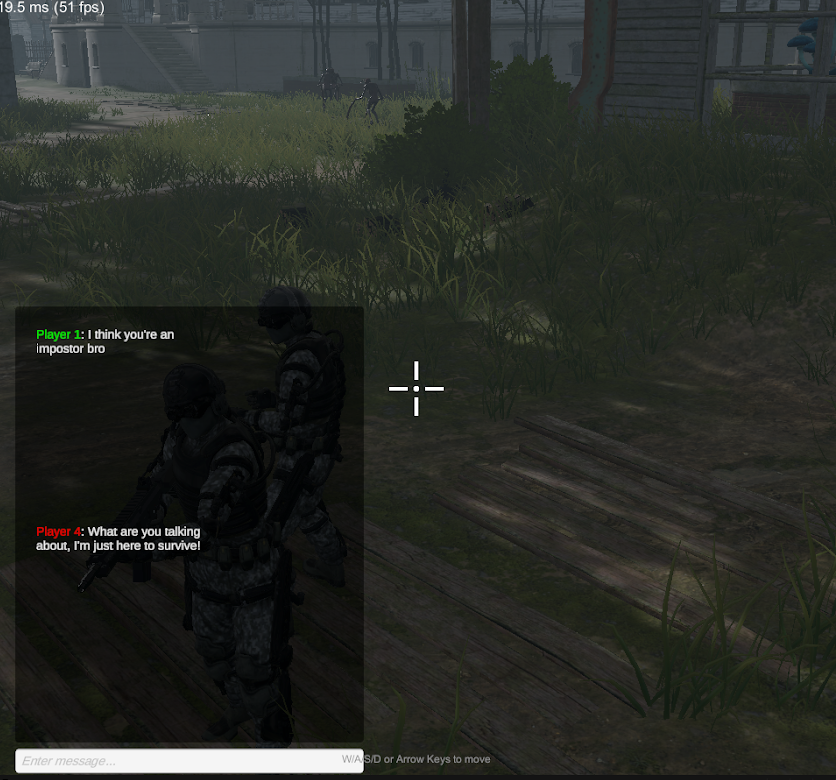
\includegraphics[width=0.85\textwidth]{Images/impostor_chat.png}
    \caption{Proximity chat during gameplay. Player 1 accuses Player 4 (the LLM impostor) of being an alien; the impostor deflects with a survival-framed denial, maintaining its cover.}
    \label{fig:impostor_chat}
\end{figure}

\subsection{Backend LLM Decision Output}

Figure~\ref{fig:backend} shows the backend terminal output captured during a live impostor reply generation. The system correctly classifies Player 1's message (\textit{``I think you're an impostor bro''}) as an \textit{accusation} with a \textit{Respond? True (1-on-1, 100\%)} decision. The LLM selects the \texttt{seed\_doubt} strategy --- described as ``weak suspicions - seeding doubt'' --- and generates the reply in \textbf{0.57 seconds}. The output fields show \textit{Style: Casual gamer}, \textit{Buffer: 7 messages}, and \textit{Facts: 1}, confirming that the memory retrieval and context assembly pipeline operated correctly before inference.

\begin{figure}[h]
    \centering
    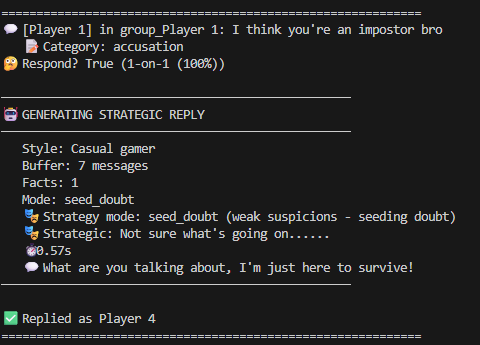
\includegraphics[width=0.85\textwidth]{Images/backend.png}
    \caption{Backend terminal output showing the LLM pipeline processing an accusation from Player 1. The system selects the \texttt{seed\_doubt} strategy and generates a reply in 0.57 seconds, styled as a casual gamer and grounded in 7 buffered messages.}
    \label{fig:backend}
\end{figure}

% -------------------------------------------------------
\section{Combat and Enemy Encounters}

\subsection{Enemy Entity}

The game world includes a hostile alien creature entity, shown in Figure~\ref{fig:enemy} in a close-quarters encounter within the Unity editor's Game view (running at 76 fps, 13.2 ms frame time). The creature is a tall, emaciated, multi-limbed organism with an elongated head and sharp appendages, rendered in a dark, desaturated colour palette consistent with the horror aesthetic. The proximity chat panel is visible on the left, indicating that combat and social interaction systems operate concurrently within the same scene.

\begin{figure}[h]
    \centering
    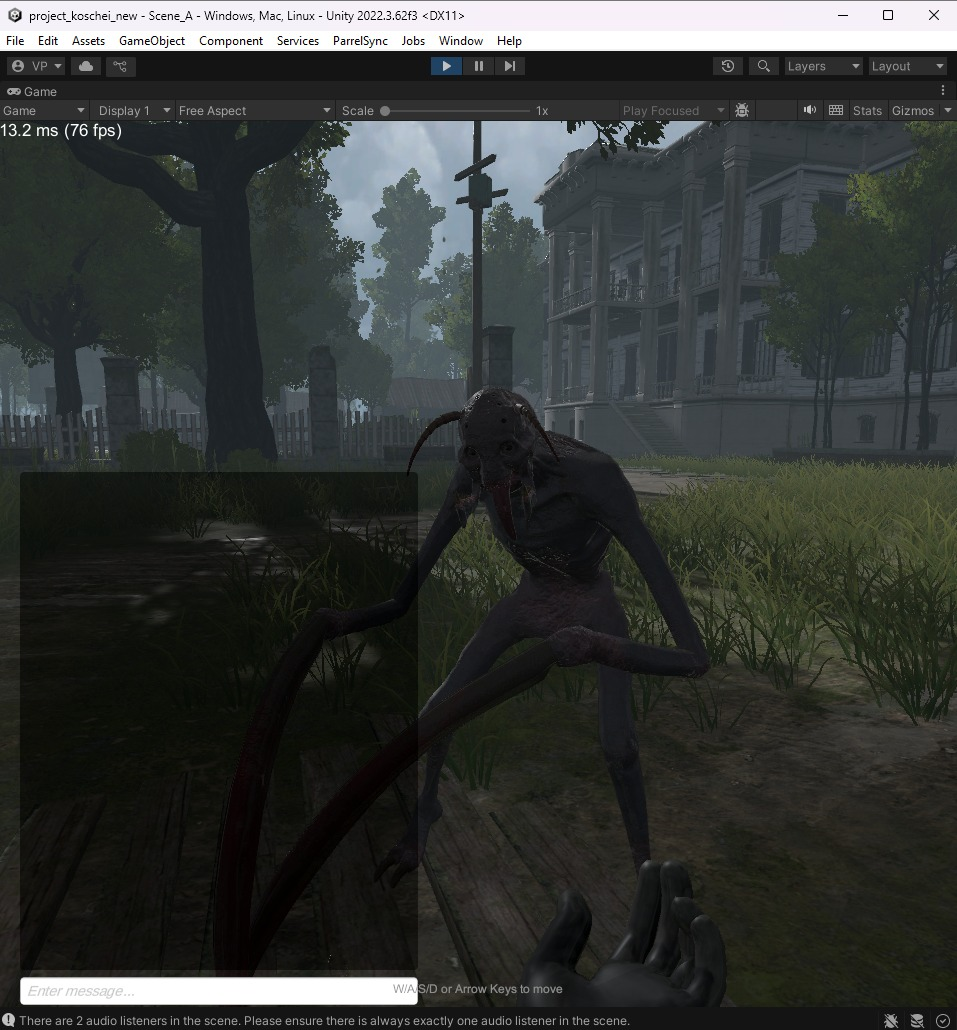
\includegraphics[width=0.85\textwidth]{Images/enemy.jpeg}
    \caption{A hostile alien creature encountered in the exclusion zone environment, running at 76 fps (13.2 ms) in the Unity editor. The entity's grotesque design reinforces the game's horror atmosphere.}
    \label{fig:enemy}
\end{figure}

\subsection{Boss Encounter}

Figure~\ref{fig:boss} depicts the boss combat encounter, tested on a white grid scene in Unity. A soldier player character armed with a rifle engages a skeletal, multi-armed boss entity at close range. The boss features a humanoid bone structure with additional articulated limbs splayed outward, presenting a visually distinct threat compared to standard enemy encounters. The crosshair is centred on the boss, and the scene confirms that the combat hit detection and player-enemy collision systems are functional.

\begin{figure}[h]
    \centering
    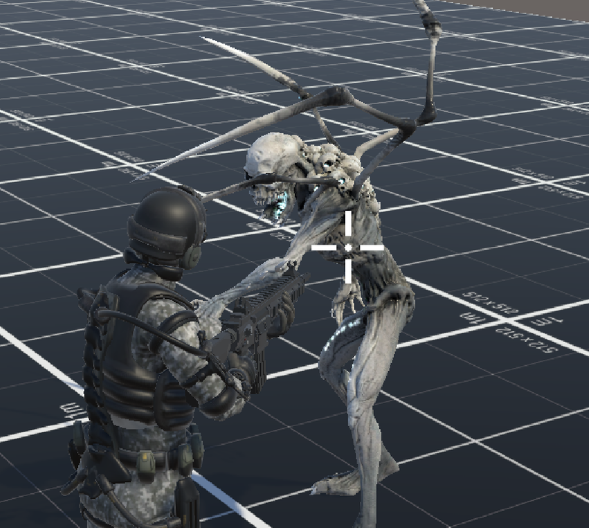
\includegraphics[width=0.85\textwidth]{Images/boss.png}
    \caption{Boss combat encounter in a Unity test scene: a soldier engages a skeletal multi-limbed boss entity at close range, demonstrating weapon aim and enemy collision systems.}
    \label{fig:boss}
\end{figure}

The results collectively demonstrate that Project Koschei delivers a functional and cohesive game experience across all implemented systems. The login and lobby flow provides smooth session management, the open-world HUD and NPC interaction systems support immersive gameplay, and the LLM-powered proximity chat --- validated by the backend terminal output showing a 0.57-second response with correct strategy selection --- achieves convincing real-time deception. Combat encounters with distinct enemy and boss entities further enrich the threat environment that underpins the game's social deduction tension.
